\documentclass{article}

\usepackage{fancyvrb}
\usepackage{pdflscape}
\usepackage{graphicx}
\usepackage{float}
\usepackage[utf8]{inputenc}
\usepackage{pmboxdraw}
\usepackage{scalerel,graphicx,xparse}
\usepackage{caption}
\usepackage{subcaption}
\usepackage{geometry}

\begin{document}

\nocite{*}

\begin{center}
\Huge 
CS2001/CS2101 Week 10 Practical

\vspace{0.5cm}

\textbf{Quicksort, Complexity and Pathological Cases}

\vspace{1cm}
\LARGE
14th November 2020

\large
\vspace{1.5cm}

\textbf{Matriculation Number: 200002548}

\vspace{0.5cm}

\textbf{Tutor: Alex Konovalov}

\end{center}

\vspace*{3cm}

\tableofcontents

\newpage
\section{Introduction}
The aim of this practical was to investigate the complexity and pathological cases surrounding the Quicksort sorting algorithm. This Quicksort implementation must be a not in-place implementation with the pivot being chosen as the last element of the list. From lectures, this is clear to be a pathological case. The metric used to describe how sorted a list is was chosen to be the edit distance, (minimum number of swaps needed to sort the list). The program should be able to generate lists according to this metric. The time it takes for Quicksort to sort generated lists of varying sortedness should then be recorded and displayed as a graph. This graph should then show the relation between sortedness and the execution time of Quicksort. Finally a conclusion should be drawn about how sortedness affects the execution time of Quicksort and how sorted a list has to be to cause a dramatic decrease in the performance of Quicksort.

\section{Design and Implementation}
Arrays were chosen as the data structure to sort as they are more efficient over lists and so could be sorted faster, this would allow me to compute results for larger arrays and larger edit distances in less time. Furthermore I could increase the number of iterations used when averaging results, without significantly impacting performance.
\subsection{Generating Lists of Varying Sortedness}
As mentioned briefly in the introduction, I defined sortedness to be the edit distance (minimum number of swaps needed to sort a list, or conversely the amount of swaps done to a sorted list to place it in its current unsorted state). This definition then allowed me to design and implement methods to create lists with a specified sortedness. The method \verb+generateSequentialIntegers()+ generates an array of sequential integers with no duplicates. The size n can be specified and the method can generate either an increasing or decreasing sequence. Elements can range from a value of \verb+0+ to \verb+n - 1+ if ascending or from \verb+n - 1+ to \verb+0+ if descending. From the definition of sortedness, a sequential array of integers is already sorted, therefore to vary the sortedness of the arrays we need to swap a elements in the array for some edit distance to decrease sortedness. This can be done with the \verb+increaseEditDistance()+ method, which swaps two random elements a total of n times to shuffle the array and increase edit distance. This shuffling allows for a sorted array to be changed into an array with a specified edit distance, since it can specify the minimum number of swaps needed for it to be sorted back into a sorted state. There is a small chance that the same element will be chosen twice randomly ($1/n^2$ chance) or that a swap will undo the swap previous to it and lead to the edit distance not increasing at all ($1/n^4$ chance), however the probability of this happening is very small and decreases with the size of the array. Therefore for suitably large arrays, this is not a significant issue.

\subsection{Quicksort Implementation}
As mentioned in the specification, a non in-place version of the Quicksort algorithm was to be implemented, with the pivot being set to the last element in the array. This leads to a time complexity on average of $O(nlog(n))$ and a worst case time complexity of $O(n^2)$ if used on an already sorted or reverse sorted array. The in-place implementation has a $O(nlog(n))$ space complexity since extra arrays are need to temporarily store elements, since the original array is not modified.

\subsection{Generating and Storing Accurate Results of Sortedness and Execution Time}
Now that we can generate lists of varying sortedness, and have provided a non in-place version of Quicksort to sort these lists, we can start to generate results for graphical analysis. 
\subsubsection{Range and Step Size of Results}
Firstly, the range of the array size and edit distance to generate results for were decided. The array size was to range from 0 to 5000, this gives a wide range to test how the execution time of Quicksort changes from the edit distance in different lengths of arrays. Furthermore, the maximum list length was set to 5000 because for arrays of size greater than that value took to long to sort (especially when their edit distance was small). The edit distance meanwhile, was to range from 0 to 100. At first it might seem logical for the edit distance to be equal to the max array size, since then you are guaranteed that nearly every element in the array has been swapped out of place. However, it turns out that as edit distance increases the gradient of execution time against edit distance decreases and the execution times remain somewhat constant past a edit distance of 50. Therefore a max edit distance of 100 was given, to properly demonstrate this decrease in gradient. A variable \verb+RESULTS_RESOLUTION+ is also used so that the edit distance and array size are iterated through with some step value so that only a certain number of results are obtained (i.e. not a result for every edit distance and every size of array). This helps to increase the efficiency of the program, since Quicksort doesn't have to be performed for specific edit distances and array lengths that are not important in the graphical analysis (since not all 0 to 5000 array sizes need to be known and displayed on a graph). \verb+ASC_SORT_ORDER+ is a boolean that can be changed to specify if ascending or descending lists should be generated. This allows the program to check the other pathological case where a reversed sorted list (in this case descending list) generates the same results.
\subsubsection{Accurately Generating and Storing Results}
Results are generated from the \verb+generateSortingResults()+ method. This method runs \verb+findMean+ \verb+SortTime()+ for an increasing edit distance and array size. The array size, edit distance and the mean sort time are stored within a list which is to be written to a csv file for graphical analysis. The method iterates through 1\% of the max array size and number of swaps each step (since \verb+RESULTS_RESOLUTION+ equals 100), this reduces the number of data points over the entire range of array lengths and number of swaps, increasing performance.\\ \\ \noindent The \verb+findMeanSortTime+ method finds the mean execution time in ms when sorting the provided array. The mean value is taken over a certain number of iterations. The method tries to remove as much error and produce as accurate results as possible. This is done using the following:
\begin{itemize}
\item warm-up iterations are used to optimise JVM code and case usage before the real test is done, increasing timing accuracy.
\item performing many timed iterations to average out the results and decrease the factor that the smallest and largest times have on the final result.
\item only timing the time that Quicksort is being performed and nothing else, so the timing is as accurate as possible.
\item shuffling the array differently each iteration, but for the same number of swaps (edit distance). This ensures that the timings obtained are not from a rare bad case scenario where a terrible swap was performed or vice versa. These are averaged out among all the possible swaps that could occur.
\item discarding the lowest and highest 10th percentile results so that only the most accurate results are left, since values significantly smaller or larger than the median are removed.
\end{itemize}
The \verb+findMeanSortTime()+ method also checks each iteration if Quicksort has worked correctly and produced a sorted array. This is done by comparing the sorted array to a generated sequential array (note that the \verb+array+ parameter passed in cannot be used to do this. This is because even though it is still a sorted sequence as Quicksort does not change the input array, the array passed in could be a reverse generated array, and the Quicksort algorithm sorts in ascending order. Therefore the arrays would not be equal as \verb+array+ would be reverse sorted and the now sorted \verb+unsorted+ array would be forward sorted.) The mean sort time in milliseconds is then calculated and returned to \verb+generateSortingResults()+ where the results are then written to a csv file for analysis.
\subsection{Graphical Analysis}
Graphical analysis was done using the \verb+matplotlib+ library in \verb+python3+. The program reads in the results from the csv file into the \verb+list_sizes+, \verb+edit_distances+ and \verb+execution_times+ arrays. The python program then generates a 3D graph of edit distance, array size and execution time to better visualise the relationship between the three variables and analyse how the execution time of Quicksort changes as sortedness decreases.
\section{Results and Conclusion}
From the results and the graph below, we can conclude that as sortedness increases, the execution time of Quicksort with the pivot being the rightmost element decreases. Initially increasing the edit distance of an already sorted array has a significant slowdown effect to the Quicksort algorithm. This can be seen for both of the pathological cases where the array is forward and revere sorted. However, after the edit distance initially increases, any further increase to the edit distance, decreases the execution time of Quicksort less and less. Therefore only a small number of swaps are needed to dramatically decrease the execution time and complexity of Quicksort from $O(n^2)$ to nearly $O(nlog(n))$, and subsequent larger edit distances have next to no effect on the execution time.\\ \\
\noindent Furthermore from the graphical analysis the changing complexity of Quicksort can be shown. The graph goes from an quadratic time complexity $O(n^2)$ where the execution time of Quicksort scales quadratically with the size of the array, to a linearithmic  $O(nlog(n))$ time complexity where execution time only scales by a logarithm of $n$ multiplied by a factor $n$. This change in complexity is singly due to the decreasing sortedness (or increasing edit distance) of the array. This complexity can be seen from the difference in scaling of the execution time of Quicksort from the small to large array sizes as the sorted array has a much steeper gradient compared to the least sorted array.


\newgeometry{left=4cm,bottom=0.8cm, right=0.1cm, top=0.8cm}
\begin{landscape}
\begin{figure}[H]
\centering
\begin{subfigure}{0.72\textwidth}
\centering
\makebox[\textwidth][c]{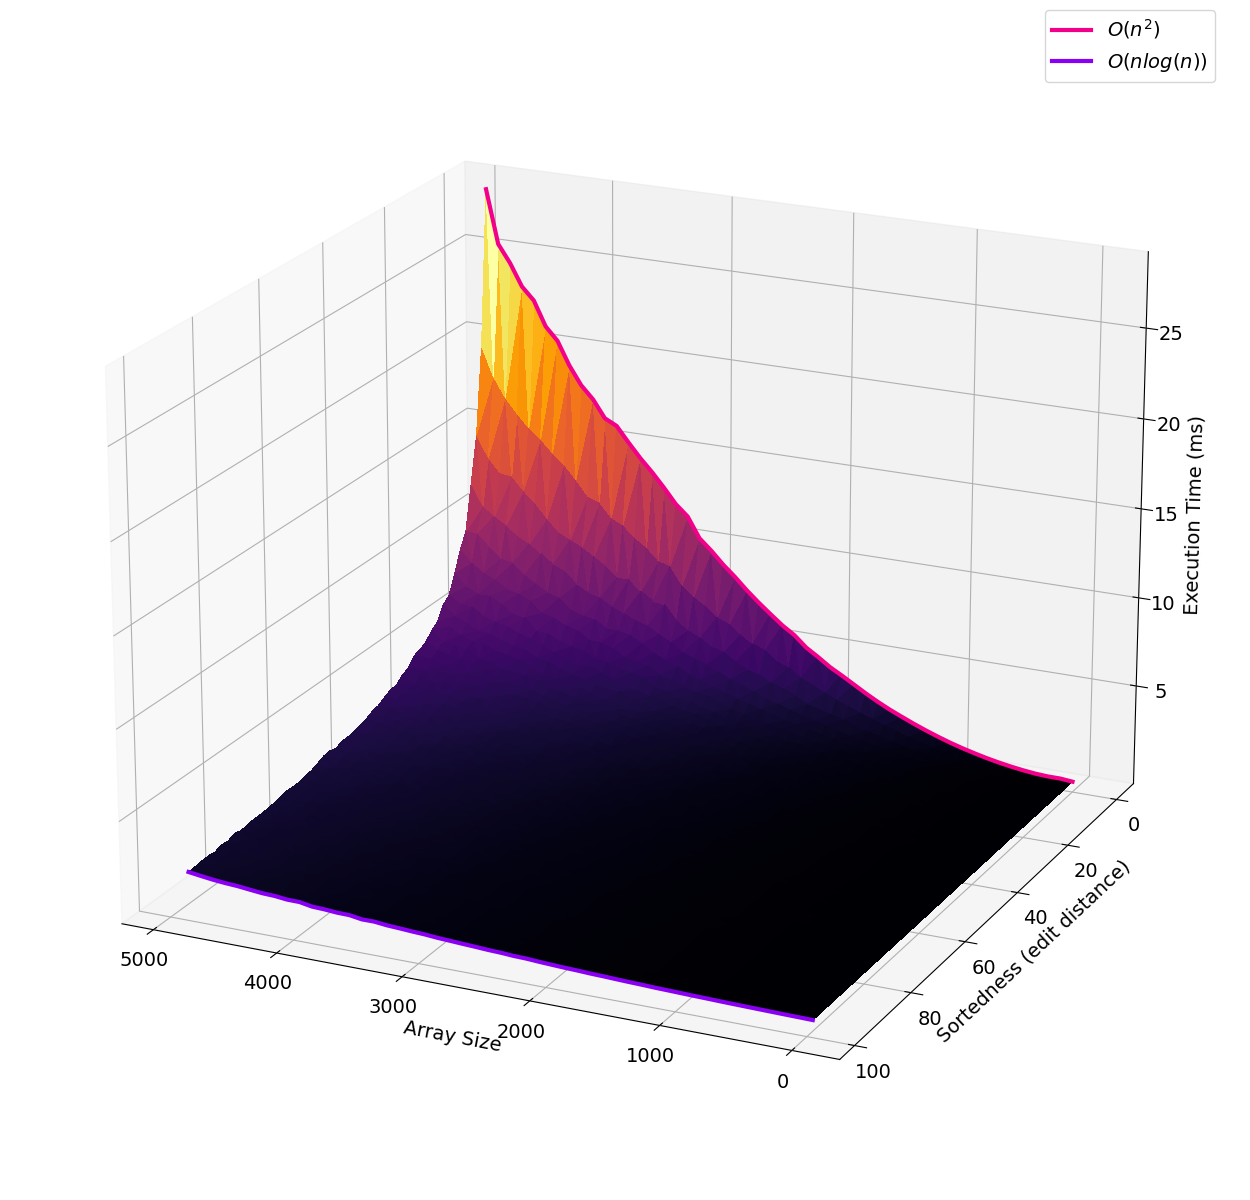
\includegraphics[width = 360px, clip]{sortedness_vs_time_vs_size.png}}
\end{subfigure}
\begin{subfigure}{0.72\textwidth}
\centering
\makebox[\textwidth][c]{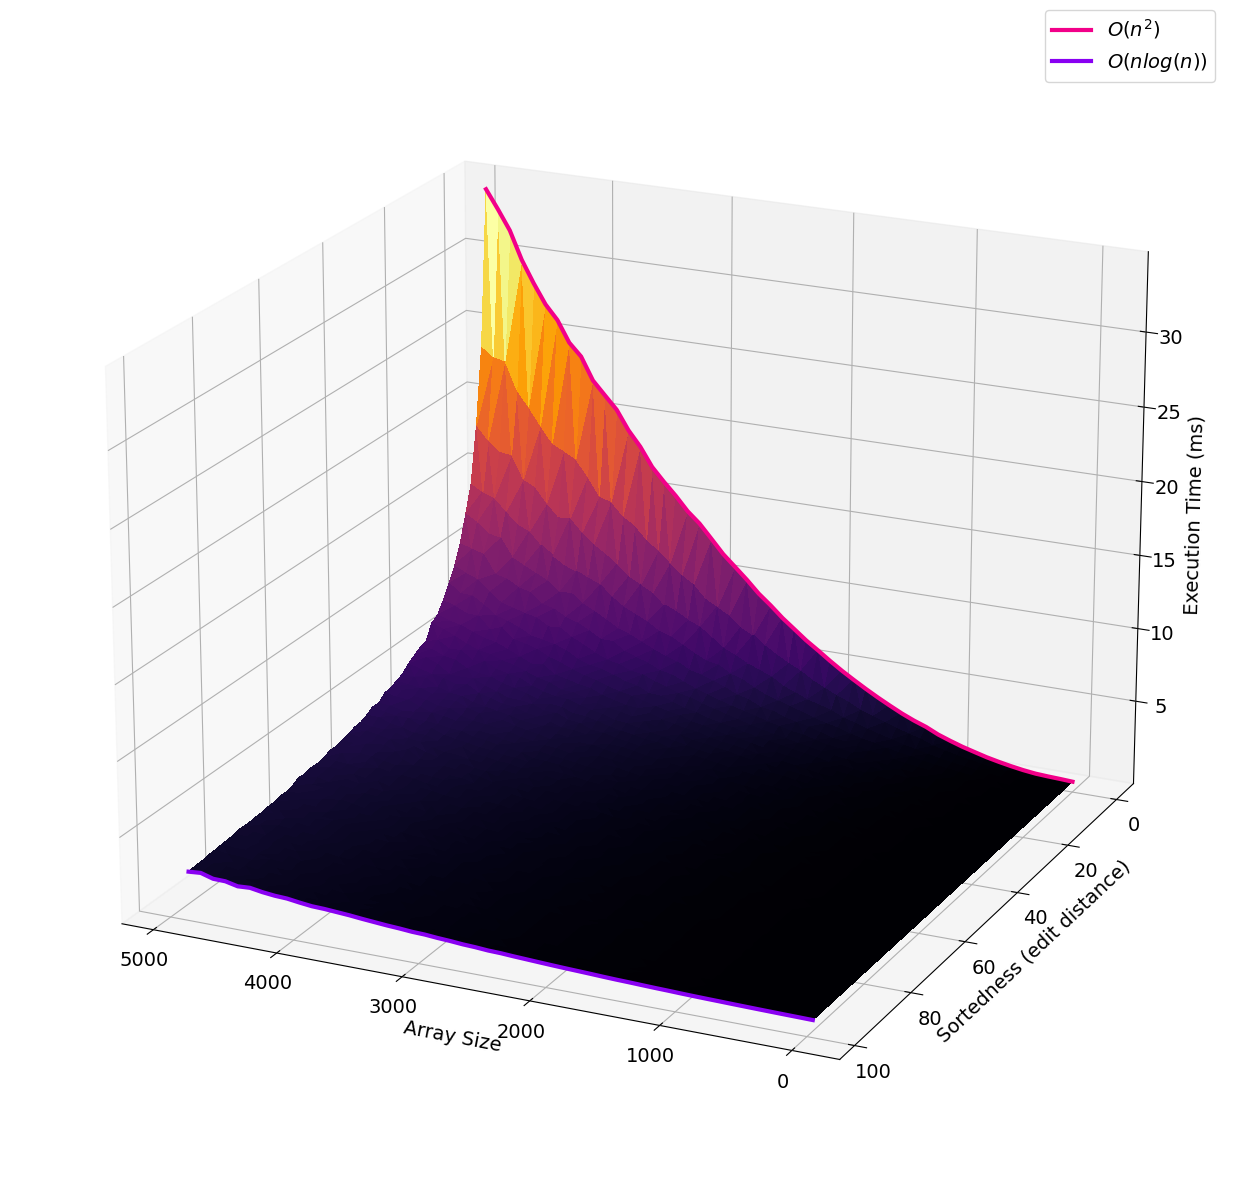
\includegraphics[width = 360px, clip]{sortedness_vs_time_vs_size_reversed.png}}
\end{subfigure}
\caption{How the execution time of Quicksort with the rightmost element as the pivot varies with edit distance and array size. Left and right graphs show how execution time varies at the forward sorted and reverse sorted pathological cases respectively. As the sortedness of the arrays decreases, Quicksorts complexity decreases from $O(n^2)$ to $O(nlog(n))$.}
\label{fig:sortedness_vs_time_vs_size}
\end{figure}
\end{landscape}
\restoregeometry

\newgeometry{left=4cm,bottom=0.8cm, right=0.1cm, top=0.8cm}
\begin{landscape}
\begin{figure}[H]
\centering
\begin{subfigure}{0.72\textwidth}
\centering
\makebox[\textwidth][c]{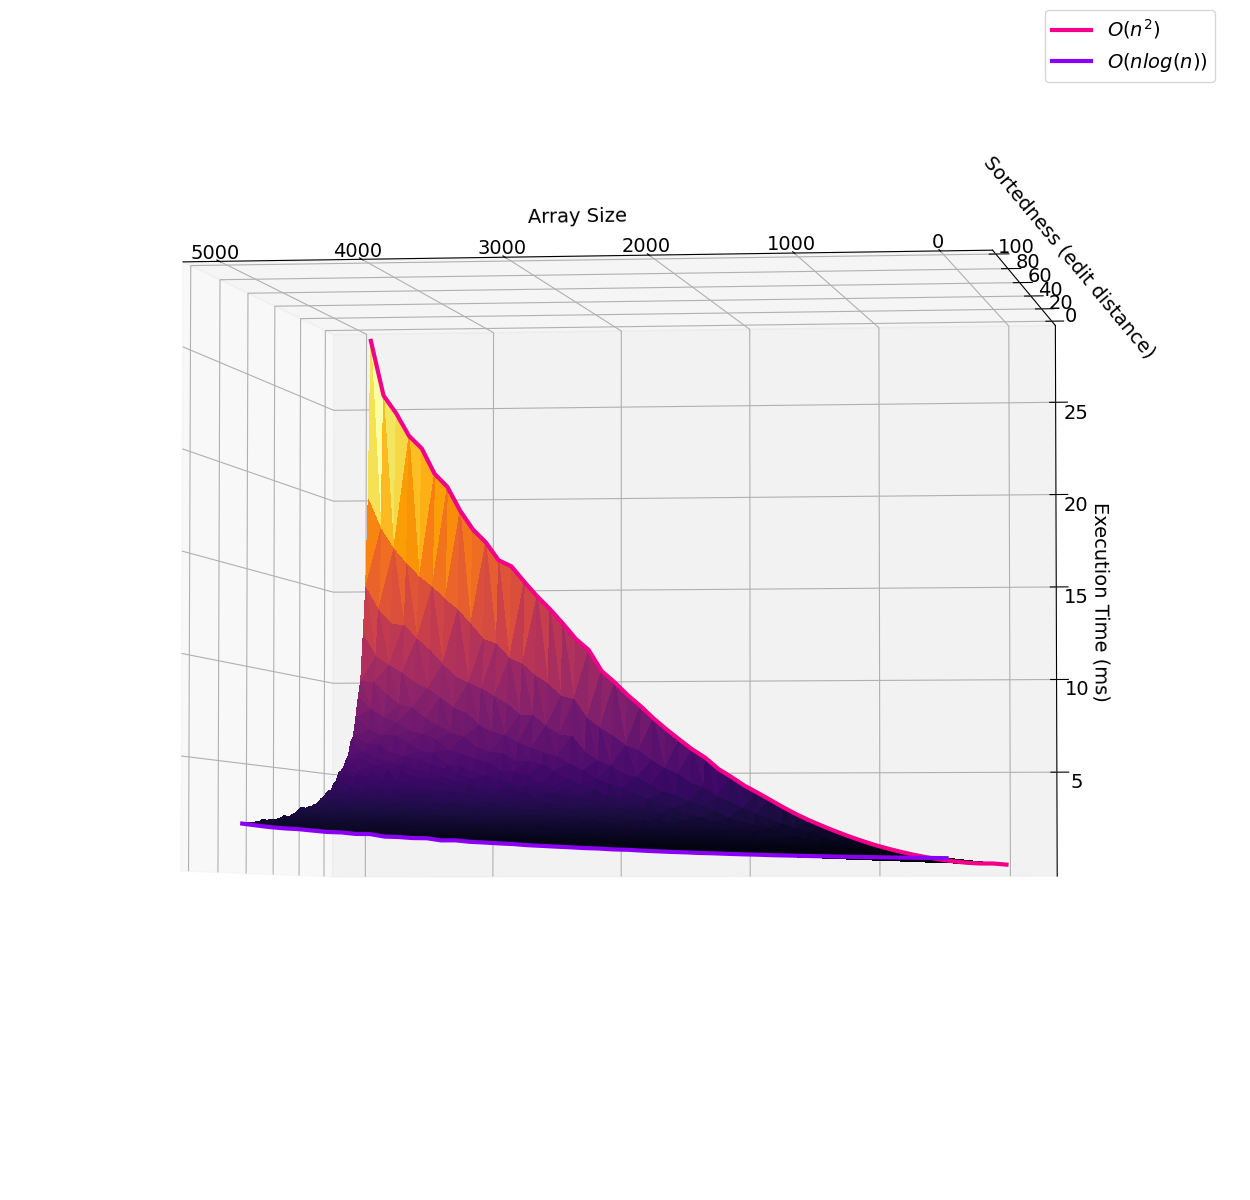
\includegraphics[width = 360px, clip]{sortedness_vs_time_vs_size_2.png}}
\end{subfigure}
\begin{subfigure}{0.72\textwidth}
\centering
\makebox[\textwidth][c]{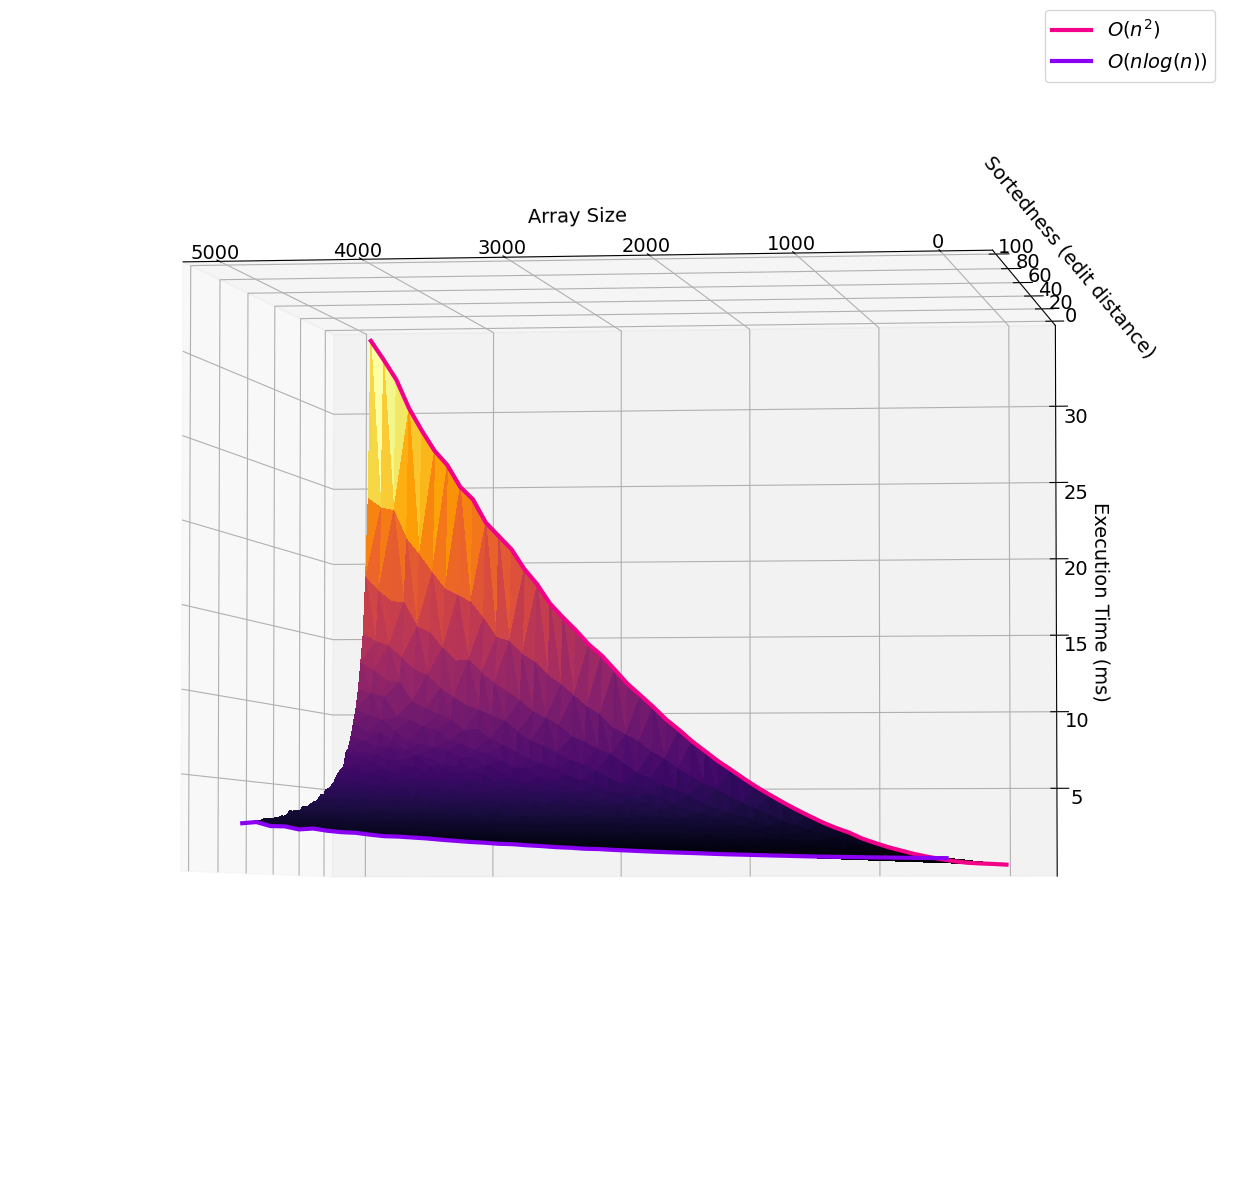
\includegraphics[width = 360px, clip]{sortedness_vs_time_vs_size_2_reversed.png}}
\end{subfigure}
\caption{An Alternative view of the surface, showing how the complexity of Quicksort with the rightmost element is a pivot is $O(n^2)$ for sorted and reverse sorted arrays. However, as the edit distance of these arrays increases, the Quicksort algorithm complexity decreases down towards a more optimal complexity of $O(nlog(n))$ and it scales much better as the size of the array increases.}
\label{fig:sortedness_vs_time_vs_size}
\end{figure}
\end{landscape}
\restoregeometry

\noindent The most challenging aspect of this practical was in obtaining accurate results of the execution time of Quicksort. It took a number of different techniques to reduce the error within the results. Moreover, performing more iterations to reduce the error proved not to be enough, since performing numerous runs of Quicksort in its pathological state was very inefficient, different techniques had to be used to reduce the error without just resorting to more iterations. \\ \\ \noindent Furthermore in this practical I have learned of the benefit if careful algorithm design to make sure pathological cases are avoided, and the advantages and disadvantages of Quicksort compared to more predictable algorithms such as Merge sort.

\begin{thebibliography}{10}
\bibitem{numeric}
Timothy Shields, \textit{Is there a way to measure how sorted a list is?}, 08-07-2013, accessed 18-11-2020, \\\texttt{https://stackoverflow.com/q/16994668}

\bibitem{numeric}
Juho, \textit{How to measure “sortedness”}, 06-05-2013, accessed 18-11-2020, \\\texttt{https://cs.stackexchange.com/q/11836}

\bibitem{numeric}
Diastrophism, \textit{How do I time a method's execution in Java?}, 07-10-2008, accessed 18-11-2020, \\\texttt{https://stackoverflow.com/q/180158}

\end{thebibliography}

\end{document}